\section{有限维近似}
\label{sec:func-finite}

Euler--Lagrange方程只在少数情形下能解出来。接下来要弄清：怎样把函数问题换成可计算的有限维问题，换完之后算出来的东西离真解有多远？本节开头的向量类比在这里变成计算方法。

\paragraph{主要思想}
可行集$\bm{C}=u_0+\bm{V}$太大，就在其中挑一个有限维的小块。取线性无关的\term{试探函数}（trial function）$\phi_1,\ldots,\phi_r\in\bm{V}$，令$\bm{V}_n$是它们张成的子空间，只在
\begin{equation}
 \bm{C}_n=u_0+\bm{V}_n
 \label{eq:func-trial}
\end{equation}
中比较候选。$\bm{V}_n$称为\term{试探空间}（trial space），$n$表示近似的精细程度。候选由系数向量$\bm{c}\in\mathbb{R}^r$决定，目标泛函变成普通的多元函数$f(\bm{c})=J(u_0+\sum_ic_i\phi_i)$。在试探空间上直接最小化目标的做法称为\term{Ritz方法}（Ritz method）。

这样得到的问题前面各章都能解，$\bm{C}_n\subseteq\bm{C}$也保证了离散最优值不低于$J^\star$。对二次目标，步骤可以完全写出来。设$J(u)=\frac12a(u,u)-\xi(u)$，$a$是对称双线性形式，$\xi$是线性泛函。代入并按$\bm{c}$整理，得到
\begin{equation}
 f(\bm{c})=J(u_0)+\frac12\bm{c}^\top\bm{A}\bm{c}-\bm{b}^\top\bm{c},
 \label{eq:func-ritz-quadratic}
\end{equation}
其中
\begin{equation}
 \bm{A}_{i,j}=a(\phi_i,\phi_j),\qquad b_i=\xi(\phi_i)-a(u_0,\phi_i).
 \label{eq:func-ritz-matrix}
\end{equation}
若$a$在$\bm{V}$上正定，$\bm{A}$对称正定，令梯度为零得到唯一的解
\begin{equation}
 \bm{c}=\bm{A}^{-1}\bm{b},\qquad \min f=J(u_0)-\frac12\bm{b}^\top\bm{c}.
 \label{eq:func-ritz-solution}
\end{equation}

最简单的例子只用一个试探函数。对$E$取$u_0=x$，$\phi_1=x(1-x)$，由式~\eqref{eq:func-phi-example}，$A_{1,1}=11/30$，$b_1=-1/12$。于是$c_1=-5/22$，这正是图~\ref{fig:func-direction-family}(b)的最小点。由式~\eqref{eq:func-ritz-solution}，目标值是
\[
 \frac23-\frac{5}{528}=\frac{347}{528}\approx0.65720.
\]
而$E^\star\approx0.65652$。一个参数就把目标差从$0.0101$降到$0.0007$。

\paragraph{计算过程}
下面用分段线性的试探函数，继续计算目标$E$，$u(0)=0$，$u(1)=1$。这时$a(v,w)=\int_0^1(v'w'+vw)\,\mathrm{d}x$，$\xi=0$。

\needspace{6\baselineskip}
\paragraph{变量}
\begin{itemize}
 \item 段数$n$，步长$\Delta=1/n$，结点$x_i=i\Delta$。例中$n=3$，$\Delta=1/3$。
 \item 帐篷函数$\phi_i$：在结点$x_i$处为$1$，其他结点为零，其间线性。自由系数$\bm{c}\in\mathbb{R}^{r}$，$r=n-1$，$c_i$就是结点$x_i$的高度。
 \item 三对角矩阵$\bm{A}\in\mathbb{R}^{r\times r}$和向量$\bm{b}\in\mathbb{R}^{r}$，由式~\eqref{eq:func-ritz-matrix}定义。
\end{itemize}

\paragraph{初始化}
取$u_0$满足边界条件。例中取右端的半个帐篷$u_0=\phi_3$，它在$x=1$处为$1$，在其余结点为零。图~\ref{fig:func-ritz-hats}(a)画了这三个函数。

\paragraph{组装与求解}
\begin{enumerate}
 \item 计算相邻帐篷的内积。每个帐篷的导数是$\pm1/\Delta$，直接积分得到
 \begin{equation}
  a(\phi_i,\phi_i)=\frac{2}{\Delta}+\frac{2\Delta}{3},\qquad a(\phi_i,\phi_{i+1})=-\frac1\Delta+\frac\Delta6,
  \label{eq:func-hat-matrix}
 \end{equation}
 不相邻的帐篷内积为零，边界上的半个帐篷$a(\phi_n,\phi_n)=\frac1\Delta+\frac\Delta3$。例中
 \[
  a(\phi_1,\phi_1)=a(\phi_2,\phi_2)=\frac{56}{9},\qquad a(\phi_1,\phi_2)=-\frac{53}{18},\qquad a(\phi_3,\phi_3)=\frac{28}{9}.
 \]
 
 \item 由式~\eqref{eq:func-ritz-matrix}组装。例中$\phi_3$只和$\phi_2$相邻，所以
 \[
  \bm{A}=\begin{bmatrix}56/9&-53/18\\-53/18&56/9\end{bmatrix},\qquad\bm{b}=\begin{bmatrix}0\\53/18\end{bmatrix}.
 \]
 
 \item 解线性方程组$\bm{A}\bm{c}=\bm{b}$。例中两边乘以$18$，得到
 \[
  112c_1-53c_2=0,\qquad-53c_1+112c_2=53.
 \]
 由第一式，$c_1=53c_2/112$。代入第二式，解得
 \[
  c_1=\frac{2809}{9735}\approx0.28855,\qquad c_2=\frac{5936}{9735}\approx0.60976.
 \]
 
 \item 由式~\eqref{eq:func-ritz-solution}计算目标值。例中$J(u_0)=\frac12a(\phi_3,\phi_3)=\frac{14}{9}$，于是
 \[
  E_3=\frac{14}{9}-\frac12\cdot\frac{53}{18}\cdot\frac{5936}{9735}\approx0.65786.
 \]
\end{enumerate}

最终得到结点高度$(0,\,0.28855,\,0.60976,\,1)$的折线。真解在相同结点的值是$0.28892$和$0.61024$，$E^\star\approx0.65652$，见图~\ref{fig:func-ritz-hats}(b)。$n$增大时，$\bm{A}$是三对角矩阵，每次求解的代价正比于$n$。

\begin{BookInlineFigure}
  \centering
  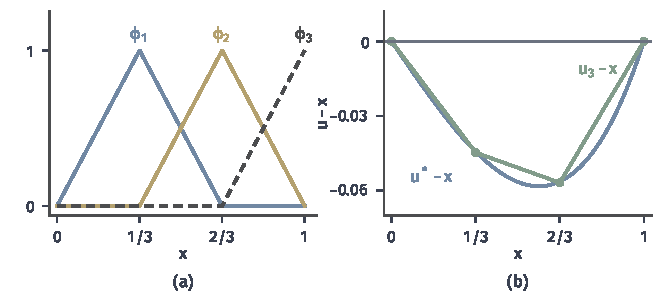
\includegraphics[width=112mm]{figures/05-optimization/08-functional-optimization/matplotlib/func-ritz-hats/figure.pdf}
  \caption{$n=3$的Ritz方法。(a)帐篷函数$\phi_1,\phi_2$是自由方向，虚线$\phi_3$用来满足$u(1)=1$。(b)为了看清差别，画的是$u-x$：蓝色为真解，绿色折线为Ritz解，结点值接近真解的结点值。}
  \label{fig:func-ritz-hats}
\end{BookInlineFigure}

\paragraph{自然边界条件不必写进试探空间}
第~\ref{sec:func-free-boundary}小节的问题中左端自由。Ritz方法的处理非常简单：不约束$x=0$处的结点，把$\phi_0$加入试探函数。条件$u'(0)=0$不写进任何地方。

$n=1$时只有一个未知数$u(0)$，$a(\phi_0,\phi_0)=4/3$，$a(\phi_0,\phi_1)=-5/6$，解得$u(0)=5/8$。这条直线的斜率不为零，自然条件并不精确成立，它要靠加密来逼近。图~\ref{fig:func-ritz-natural}中，$n=3$时左端第一段的斜率降到$0.110$，$u(0)=0.6457$，真解是$1/\cosh1\approx0.6481$。目标值$0.4063$、$0.3835$也逐步接近$E^\star\approx0.3808$。

\begin{BookInlineFigure}
  \centering
  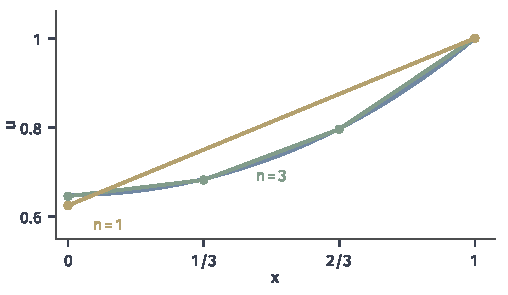
\includegraphics[width=86mm]{figures/05-optimization/08-functional-optimization/matplotlib/func-ritz-natural/figure.pdf}
  \caption{左端自由时的Ritz解。蓝色是真解$\cosh x/\cosh1$，黄色是$n=1$，绿色是$n=3$。试探空间没有写入$u'(0)=0$，第一段的斜率随加密而趋于零。}
  \label{fig:func-ritz-natural}
\end{BookInlineFigure}

先离散再优化，和先写出方程再离散，是两条路线。对$E$，后者用差分代替二阶导数，内部结点的方程是$\frac1\Delta(-u_{i-1}+2u_i-u_{i+1})+\Delta u_i=0$，而Ritz方法的$\Delta u_i$项换成了$\frac\Delta6(u_{i-1}+4u_i+u_{i+1})$。$n=3$时，差分解的结点值是$0.28929$和$0.61071$，精度相当。差别在于结构：Ritz方法的矩阵自动对称，目标值从上方逼近$E^\star$，自然边界条件自动处理；差分方法要为边界单独设计格式。

\paragraph{三种误差}
算出的结果与真解的距离由几件不同的事情决定，必须分开。下面逐一说明，它们的区别列在表~\ref{tab:func-errors}中。

第一件事是固定函数能否被逼近：给定一个$v\in\bm{C}$，$\bm{C}_n$中有没有函数$v_n$，使$J(v_n)\to J(v)$。这是试探空间和目标的性质，与优化无关。例如$v=x+\frac14\sin2\pi x$，取它的线性插值$v_n$，$\lvert E(v_n)-E(v)\rvert$按$n^{-2}$衰减，见图~\ref{fig:func-three-errors}(a)的黄线。

第二件事是离散极小者$u_n$是否收敛到真解，这要求$J(u_n)\to J^\star$，还要求$u_n$本身收敛。它比第一件事多要求目标有存在性论证那样的结构。第三件事是数值求解误差：实际算出的$\tilde{u}_n$与精确的离散极小者$u_n$之间的差。

\begin{BookInlineTable}
  \centering
  \caption{三种误差。}
  \label{tab:func-errors}
  \begin{tabular}{lll}
    \toprule
    误差 & 比较的对象 & 决定因素\\
    \midrule
    固定函数逼近 & $J(v_n)$ 与 $J(v)$ & 试探空间、$J$ 的连续性\\
    离散极小者收敛 & $u_n$ 与 $u^\star$ & 上一项及存在性结构\\
    数值求解 & $\tilde{u}_n$ 与 $u_n$ & 算法与迭代步数\\
    \bottomrule
  \end{tabular}
\end{BookInlineTable}

\paragraph{二次目标：Ritz解是能量范数下的最佳逼近}
对二次目标，第二件事可以精确回答。目标值的差恰好是一个距离的平方，下面的定理把“目标最小”变成“离真解最近”。

\begin{theorem}[Ritz方法的最佳逼近性质]
\label{thm:func-cea}
设$\bm{V}$是Hilbert空间，$a$是$\bm{V}$上的对称双线性形式，存在$0<\mu\leq L$，使
\begin{equation}
 \mu\lVert\eta\rVert^2\leq a(\eta,\eta)\leq L\lVert\eta\rVert^2\qquad(\eta\in\bm{V}),
 \label{eq:func-a-bounds}
\end{equation}
并且$J(u)=\frac12a(u,u)-\xi(u)$在$\bm{C}=u_0+\bm{V}$上有极小点$u^\star$。则对$v\in\bm{C}$，
\begin{equation}
 J(v)-J(u^\star)=\frac12a(v-u^\star,v-u^\star).
 \label{eq:func-energy-identity}
\end{equation}
若$u_n$是$J$在$\bm{C}_n=u_0+\bm{V}_n$上的极小点，则
\begin{equation}
 a(u_n-u^\star,\,u_n-u^\star)=\min_{v\in\bm{C}_n}a(v-u^\star,\,v-u^\star),
 \label{eq:func-cea}
\end{equation}
并且
\begin{equation}
 \lVert u_n-u^\star\rVert\leq\sqrt{\frac{L}{\mu}}\,\min_{v\in\bm{C}_n}\lVert v-u^\star\rVert.
 \label{eq:func-cea-norm}
\end{equation}
\end{theorem}

\begin{proof}
令$\eta=v-u^\star\in\bm{V}$，把$J(u^\star+\eta)$按$\eta$展开：
\[
 J(u^\star+\eta)-J(u^\star)=DJ(u^\star)[\eta]+\frac12a(\eta,\eta).
\]
由式~\eqref{eq:func-stationary}，一次项为零，得到式~\eqref{eq:func-energy-identity}。

$u_n$使左端在$\bm{C}_n$上最小，也就使$a(v-u^\star,v-u^\star)$最小，这就是式~\eqref{eq:func-cea}。对任意$v\in\bm{C}_n$，由$a$的两个界，
\[
 \mu\lVert u_n-u^\star\rVert^2\leq a(u_n-u^\star,u_n-u^\star)\leq a(v-u^\star,v-u^\star)\leq L\lVert v-u^\star\rVert^2.
\]
开方并对$v$取最小，得到式~\eqref{eq:func-cea-norm}。
\end{proof}

式~\eqref{eq:func-energy-identity}的直观是：能量地形是一只以$u^\star$为底的碗，比较目标值就是比较到碗底的距离。式~\eqref{eq:func-cea}说明，Ritz方法不需要事先知道$u^\star$，却自动选出了$u^\star$在试探空间中的最佳逼近。在式~\eqref{eq:func-energy}的例子上，$a$就是$H^1$内积，$\mu=L=1$，Ritz解是$u^\star$在$H^1$范数下的正交投影。

这也把收敛速度转化成逼近问题。线性元逼近$H^1$函数的误差按$\Delta$衰减，目标差是距离的平方，按$\Delta^2$衰减。图~\ref{fig:func-three-errors}(a)的绿线实测：$n=16,32,64$时目标差为$4.79\times10^{-5}$、$1.20\times10^{-5}$、$3.00\times10^{-6}$，每次缩小到四分之一。

\begin{BookInlineFigure}
  \centering
  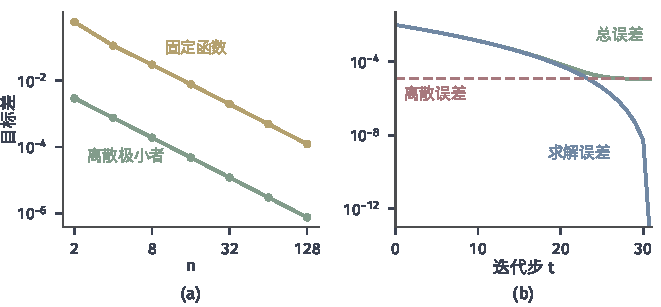
\includegraphics[width=112mm]{figures/05-optimization/08-functional-optimization/matplotlib/func-three-errors/figure.pdf}
  \caption{目标$E$的三种误差。(a)黄色是固定函数$x+\frac14\sin2\pi x$的线性插值的能量误差，绿色是Ritz解的目标差$E(u_n)-E^\star$，两者都按$n^{-2}$衰减。(b)$n=32$时用共轭梯度法从$u=x$出发：蓝色是求解误差$E(\tilde{u}_n)-E(u_n)$，绿色是总误差$E(\tilde{u}_n)-E^\star$，红色虚线是离散误差$1.20\times10^{-5}$。}
  \label{fig:func-three-errors}
\end{BookInlineFigure}

\paragraph{一般目标的收敛}
对非二次的目标，能保证的结论要弱一些，证明正好回用第~\ref{sec:func-existence}节的论证。这里用$\tilde{u}_n$同时把求解误差包括进来。

\begin{theorem}[Ritz方法的收敛]
\label{thm:func-ritz-convergence}
设$X$、$\bm{C}$和$J$满足定理~\ref{thm:func-direct-method}中反射、弱序列闭和弱序列下半连续的条件，$J$的每个下水平集都有界，$J$在$\bm{C}$上按范数连续且处处有限，$\bm{C}_n\subseteq\bm{C}$非空。设对每个$v\in\bm{C}$，存在$v_n\in\bm{C}_n$使$v_n\to v$。若$\tilde{u}_n\in\bm{C}_n$满足
\begin{equation}
 J(\tilde{u}_n)\leq\inf_{\bm{C}_n}J+\varepsilon_n,\qquad\varepsilon_n\to0,
 \label{eq:func-approx-minimizer}
\end{equation}
则$J(\tilde{u}_n)\to J^\star$，$\tilde{u}_n$有弱收敛子列，且每个弱收敛子列的极限都是最优解。
\end{theorem}

\begin{proof}
任取$\varepsilon>0$和$v\in\bm{C}$，使$J(v)\leq J^\star+\varepsilon$。取$v_n\to v$，由连续性$J(v_n)\to J(v)$。由式~\eqref{eq:func-approx-minimizer}，
\[
 J^\star\leq J(\tilde{u}_n)\leq J(v_n)+\varepsilon_n.
\]
令$n\to\infty$，再令$\varepsilon\to0$，得到$J(\tilde{u}_n)\to J^\star$。所以$\tilde{u}_n$是极小化序列。

下水平集有界，所以序列有界，由反射性有弱收敛子列。设某子列弱收敛到$u$，$\bm{C}$弱序列闭给出$u\in\bm{C}$，弱序列下半连续给出$J(u)\leq J^\star$，所以$u$是最优解。
\end{proof}

定理说明Ritz方法产生的是一个极小化序列，第~\ref{sec:func-existence}节的三关同时决定了它的命运。若$J$还满足$J(v)-J^\star\geq\frac\mu2\lVert v-u^\star\rVert^2$，例如$J$是$\mu$-强凸的，则目标收敛蕴含范数收敛。

\paragraph{各条件的作用}
条件去掉，结论就会失败。连续性保证“固定函数的能量能被逼近”。若$J$不连续，$\bm{C}_n$稠密也不够：存在目标使得Lipschitz函数上的下确界严格大于$W^{1,1}$上的下确界，这称为Lavrentiev现象，经典例子是Manià给出的。这时分段线性的试探函数永远达不到真正的下确界，证明较长，读者可查阅变分法的专著。

弱序列下半连续保证极限真的最优。对目标~\eqref{eq:func-bolza}，取$n$为偶数的线性元，结点值交替取$0,\Delta,0,\Delta,\ldots$的折线就是图~\ref{fig:func-bolza-zigzag}的锯齿，所以
\[
 0<\min_{\bm{C}_n}J\leq\frac{\Delta^2}{3}.
\]
每个离散问题都有解，最优值也收敛到$J^\star=0$，离散解的振幅趋于零，一致趋于$u=0$。但$J(0)=1$，这个极限根本不是解，原问题也没有解。计算机算出的“收敛”数字，不能代替第~\ref{sec:func-existence}节的存在性论证。

\paragraph{数值求解误差}
对二次目标，由式~\eqref{eq:func-energy-identity}（把它用在$\bm{C}_n$上，$u_n$代替$u^\star$），两种误差恰好相加：
\begin{equation}
 J(\tilde{u}_n)-J^\star=\frac12a(\tilde{u}_n-u_n,\tilde{u}_n-u_n)+\bigl(J(u_n)-J^\star\bigr).
 \label{eq:func-error-split}
\end{equation}
第一项是求解误差，第二项是离散误差。图~\ref{fig:func-three-errors}(b)中，共轭梯度法的总误差下降到约$25$步后就贴住了离散误差，再多的迭代只减少第一项。所以迭代的停止精度应该与离散误差相称，把线性方程组解到机器精度是浪费。

矩阵$\bm{A}$的条件数按$n^2$增长，这是第~\ref{sec:func-hilbert-gradient}小节讲过的现象。用刚度矩阵作预条件，相当于换成$H^1$型内积，迭代次数就基本不随网格变化。

\paragraph{非二次目标}
非二次目标的离散问题用前面各章的方法求解，第~\ref{chap:second-order-methods}章的牛顿法尤其合适。考虑
\[
 J(u)=\int_0^1\Bigl(\frac12u'(x)^2+\frac14u(x)^4\Bigr)\,\mathrm{d}x,\qquad u(0)=0,\ u(1)=1.
\]
它满足定理~\ref{thm:func-tonelli}，又是严格凸的，解存在且唯一。取$u=x+c\,x(1-x)$，用Beta积分把$x^4(1+c(1-x))^4$逐项积分，得到一元多项式
\[
 f(c)=\frac{11}{20}+\frac{c}{30}+\frac{19}{105}c^2+\frac{c^3}{280}+\frac{c^4}{2520}.
\]

从$c^{(0)}=0$出发用牛顿法。第一步，$f'(0)=\frac1{30}$，$f''(0)=\frac{38}{105}$，于是
\[
 c^{(1)}=-\frac{7}{76}\approx-0.09211.
\]
第二步，$f'(c^{(1)})\approx8.97\times10^{-5}$，$f''(c^{(1)})\approx0.35997$，于是
\[
 c^{(2)}\approx-0.09235.
\]
此时$f\approx0.548462$，比$f(0)=0.55$低，再迭代目标值几乎不变。

对线性元离散的完整问题，牛顿法的Hessian是三对角的，每步代价正比于$n$。图~\ref{fig:func-newton-mesh}中，$n=8,32,128$的三条残差曲线几乎重合，都在$3$步内到达机器精度，这称为网格无关性。这个性质表明，牛顿法的步数是函数问题本身的性质，而不是某个离散向量问题的性质。

\begin{BookInlineFigure}
  \centering
  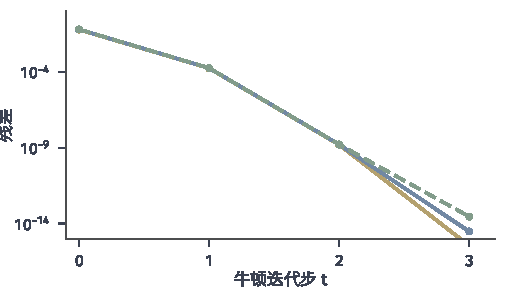
\includegraphics[width=86mm]{figures/05-optimization/08-functional-optimization/matplotlib/func-newton-mesh/figure.pdf}
  \caption{牛顿法的网格无关性。目标$\int_0^1(\frac12u'^2+\frac14u^4)\,\mathrm{d}x$，从$u=x$出发，线性元、梯形求积。纵轴是在$\bm{K}^{-1}$范数下度量的梯度残差，$\bm{K}$是刚度矩阵，它对应函数空间的对偶范数。黄、蓝、绿虚线分别是$n=8,32,128$，三条线几乎重合。}
  \label{fig:func-newton-mesh}
\end{BookInlineFigure}
